% Lancaster et. al. Solutions Manual

\documentclass{report}
\usepackage[paperwidth=18cm, paperheight=23.6 cm, top = 20mm, bottom = 18mm, left=10mm, right = 10mm]{geometry}
\usepackage{fancyhdr}
\pagestyle{fancy}

\renewcommand{\chaptermark}[1]{%
\markboth{\chaptername
\ \thechapter.\ #1}{}}


\usepackage{graphicx}
\usepackage{amsmath, amsfonts, amssymb, amsthm}
\usepackage{tensor}
\usepackage{physics}
\usepackage{cancel}
\usepackage{hyphenat}
\usepackage{hyperref}
\hypersetup{colorlinks, linkcolor = [RGB]{66, 128, 128}, urlcolor = red, linktocpage = true}
\usepackage{enumitem}

% \usepackage{charter}

\DeclareMathOperator{\arctanh}{arctanh}

\newlist{subquests}{enumerate}{2}
\setlist[subquests, 1]{leftmargin=*, label = \textbf{\arabic*.}}
\setlist[subquests, 2]{leftmargin=*, label = (\alph*)}

\renewcommand{\familydefault}{\sfdefault}
\usepackage{tkz-euclide}
\usepackage{tikz}

\usepackage{etoolbox} % provides \patchcmd macro
\makeatletter % modify the "headings" page style
\patchcmd{\ps@headings}{{\slshape\rightmark}\hfil\thepage}{\thepage\hfil}{}{}
\makeatother
\pagestyle{headings}  % load the (re-defined) "headings" page style (default: "plain")

\usetikzlibrary{calc,arrows}
\usetkzobj{all}
\theoremstyle{definition}

\usetikzlibrary{decorations.markings}

\usepackage{color}
\definecolor{mygrey}{gray}{0.1}
\color{mygrey}

\newtheorem{chapter1}{Exercise}
\newcounter{subpart1}[chapter1]

\begin{document}

\title{Solutions to \\Principles of Quantum Mechanics (Second Edition)\\ by Ramamurti Shankar}
\date{}
\author{Arjit Seth}

\maketitle

\chapter{Mathematical Introduction}

\begin{chapter1}\label{prob:1}
	The null vector is $(0,0,0)$. The inverse under addition is $(-a,-b,-c)$. A vector of the form $(a,b,1)$ does not form a vector space because it fails to satisfy the closure property under addition and multiplication:
	\begin{gather*}
		(a,b,1) + (d,e,1) = (a+d, b+e, 2) \notin (a,b,1) \\
		\alpha(a,b,1) = (\alpha a, \alpha b, \alpha) \notin (a,b,1)
	\end{gather*}
	
\end{chapter1}

\begin{chapter1}\label{prob:2}
	
\end{chapter1}

\begin{chapter1}\label{prob:3}
	The set of kets is not linearly independent, as $\ket 3 = \ket 1 -2\ket 2$.
\end{chapter1}

\begin{chapter1}\label{prob:4}
	Arrange the row vectors into a matrix and find the determinant:
		\begin{gather*}
			\begin{vmatrix}
				1 & 1 & 0 \\
				1 & 0 & 1 \\
				3 & 2 & 1 
			\end{vmatrix}
			= 0
		\end{gather*}
		Since the determinant is zero, one of the row vectors is expressible as a linear combination of the others. This is seen in $(3,2,1) = 2(1,1,0) + (1,0,1)$. \\\\
		For the second set of vectors, we perform the same procedure:
		\begin{gather*}
			\begin{vmatrix}
				1 & 1 & 0 \\
				1 & 0 & 1 \\
				0 & 1 & 1
			\end{vmatrix}
			= 2
		\end{gather*}
		So there is no vector in this set that is expressible as a linear combination of the other vectors.\\\\
\end{chapter1}

\begin{chapter1}\label{prob:5}
	Let $\ket {\mathrm{I}} = \va{A}$ and $\ket{\mathrm{II}} = \va B$. Following Gram-Schmidt orthonormalisation:
		\begin{gather*}
			\hat {\bf A} = \frac{3}{5}{\hat {\bf i}} + \frac{4}{5}{\hat {\bf j}} = \ket 1
		\end{gather*}
		\begin{gather*}
			\ket {2'} = \ket{\mathrm{II}} - \ket 1 \braket{1}{\mathrm{II}} = \frac{18}{5} 
		\end{gather*}
\end{chapter1}

\begin{chapter1}\label{prob:6}
	
\end{chapter1}

\begin{chapter1}\label{prob:7}
	
\end{chapter1}

\newtheorem{chapter2}{Exercise}
\newcounter{subpart2}[chapter2]

\chapter{Review of Classical Mechanics}

\begin{chapter2}\label{prob: 1}
	The Lagrangian of the system is:
		\begin{gather*}
			\mathcal{L} = \frac{1}{2}m{\dot x}^2 - \frac{1}{2}kx^2
		\end{gather*}
		Solving the Euler-Lagrange equation gives the equation of motion:
		\begin{gather*}
			\dv{t}\pdv{\mathcal{L}}{\dot x} - \pdv{\mathcal{L}}{x}
			= m\ddot x + kx = 0
		\end{gather*}
\end{chapter2}

\begin{chapter2}\label{prob: 2}
	The Lagrangian of the system is:
		\begin{gather*}
			\mathcal{L} = \frac{1}{2}m{\dot x}^2_1 + \frac{1}{2}m{\dot x}^2_2 - \frac{1}{2}k(x^2_1 + x^2_2) - \frac{1}{2}k(x_1 - x_2)^2
		\end{gather*}
		Solving the Euler-Lagrange equations gives the equations of motion:
		\begin{gather*}
			\dv{t} \pdv{\mathcal{L}}{\dot x_1} - \pdv{\mathcal{L}}{x_1}
			= m{\ddot x_1} + 2kx_1 - kx_2 =0 
		\end{gather*}
		\begin{gather*}
			\dv{t} \pdv{\mathcal{L}}{\dot x_2} - \pdv{\mathcal{L}}{x_2}
			= m{\ddot x_2} + 2kx_2 - kx_1 =0 
		\end{gather*}
		Rearranging, we get the same equations of motion:
		$$ \ddot x_1 = -\frac{2k}{m}x_1 + \frac{k}{m}x_2 $$
		$$ \ddot x_2 = \frac{k}{m}x_1 - \frac{2k}{m}x_2 $$
\end{chapter2}

\begin{chapter2}\label{prob: 3}
	The Lagrangian in polar coordinates is:
		\begin{gather*}
			\mathcal{L} = \frac{1}{2}m \abs{\dot {\bf r}}^2 - V(r) = \frac{1}{2}m \bqty{\dot r^2 + r^2\dot\theta^2 + (r^2\sin^2\theta)\dot\phi^2} - V(r)  
		\end{gather*}
		Solving the Euler-Lagrange equations gives the equations of motion:
		\begin{gather*}
			\dv{t}\pdv{\mathcal{L}}{\dot r} - \pdv{\mathcal{L}}{r} = m\ddot r - mr\dot\theta^2 - (mr\sin^2\theta)\dot\phi^2 + \pdv{V}{r} = 0
		\end{gather*}
		\begin{gather*}
			\dv{t}\pdv{\mathcal{L}}{\dot \theta} - \pdv{\mathcal{L}}{\theta} = mr^2\ddot\theta + 2mr\dot r \dot\theta - \frac{1}{2}(mr^2\sin 2\theta)\dot\phi^2 = 0
		\end{gather*}
		\begin{gather*}
			\dv{t}\pdv{\mathcal{L}}{\dot \phi} - \pdv{\mathcal{L}}{\phi}
			= (mr^2\sin^2\theta)\ddot\phi + 2m\dot\phi(r\dot r \sin^2\theta + r^2\dot\theta\sin 2\theta) = 0
			\end{gather*}
\end{chapter2}

\begin{chapter2}\label{prob: 4}
	Substituting ${\bf \dot r}_1$ and ${\bf \dot r}_2$ with ${\bf \dot r_{\mathrm{CM}}}$ and ${\bf \dot r}$:
	\begin{gather*}
		\mathcal{L} = \frac{1}{2}m_1\left|{\bf \dot r_{\mathrm{CM}}} + \frac{m_2{\bf \dot r}}{m_1 + m_2}\right|^2 + \frac{1}{2}m_2\left|{\bf \dot r_{\mathrm{CM}}} - \frac{m_1{\bf \dot r}}{m_1 + m_2}\right|^2 - V({\bf r})
	\end{gather*}
	Expanding the squares:
	\begin{align}
		\mathcal{L} = \frac{1}{2}(m_1 + m_2)\left|{\bf \dot r_{\mathrm{CM}}}\right|^2 + \frac{1}{2}m_1\left|\frac{2m_2{\bf \dot r r_{\mathrm{CM}}}}{m_1 + m_2}\right| + \frac{1}{2}m_1\pqty{\frac{m_2}{m_1 + m_2}}^2\left|{\bf \dot r}\right|^2 \notag\\ 
		- \frac{1}{2}m_2\left|\frac{2m_1{\bf \dot r r_{\mathrm{CM}}}}{m_1 + m_2}\right| + \frac{1}{2}m_2\pqty{\frac{m_1}{m_1 + m_2}}^2\left|{\bf \dot r}\right|^2 - V({\bf r}) 
	\end{align}
	Which gives the final expression:
	\begin{gather*}
		\mathcal{L} = \frac{1}{2}(m_1 + m_2)\left|{\bf \dot r_{\mathrm{CM}}}\right|^2 + \frac{1}{2}\frac{m_1 m_2}{m_1 + m_2}|{\bf \dot r}|^2 - V({\bf r})
	\end{gather*}
\end{chapter2}

\begin{chapter2}\label{prob: 5}
	
\end{chapter2}

\begin{chapter2}\label{prob: 6}
	The conservation of energy in the harmonic oscillator states that:
		\begin{gather*}
			\frac{p^2}{2m} + \frac{1}{2}kx^2 = E
		\end{gather*}
		Dividing both sides by $E$:
		\begin{gather*}
			\frac{p^2}{2mE} + \frac{kx^2}{2E}= 1 \longrightarrow \pqty{\frac{x}{a}}^2 + \pqty{\frac{p}{b}}^2 = 1, \;\; a^2 = \frac{2E}{k}\;\;, \;\;b^2 = 2mE
		\end{gather*}
\end{chapter2}

\begin{chapter2}\label{prob: 7}
	The Lagrangian of the system is:
		\begin{gather*}
			\mathcal{L} = \frac{1}{2}m{\dot x}^2_1 + \frac{1}{2}m{\dot x}^2_2 - \frac{1}{2}k(x^2_1 + x^2_2) - \frac{1}{2}k(x_1 - x_2)^2
		\end{gather*}
		Finding the generalised momenta:
		\begin{gather*}
			p_i = \pdv{\mathcal{L}}{\dot x_i} = m_i \dot x_i \longrightarrow \dot x_i = \frac{p_i}{m_i}
		\end{gather*}
		The Hamiltonian is found by:
		\begin{gather*}
			\mathcal{H} = \sum_i p_i \dot x_i - \mathcal{L} = \mathcal{T+V} = \frac{p^2_1}{2m} + \frac{p^2_2}{2m} + \frac{1}{2}k(x^2_1 + x^2_2) + \frac{1}{2}k(x_1 - x_2)^2
		\end{gather*}
		Solving Hamilton's equations gives the equations of motion:
		\begin{gather*}
			\pdv{\mathcal{H}}{p_i} = \dot x_i \longrightarrow \dot x_i = \frac{p_i}{m_i}
	 	\end{gather*}
	 	\begin{gather*}
	 		-\pdv{\mathcal{H}}{x_i} = \dot p_i \longrightarrow \dot p_1 = - 2kx_1 + kx_2, \;\; \dot p_2 = kx_1 - 2kx_2
	 	\end{gather*}
	 	But $\dot p_i = m\ddot x_i$, so we get the same equations of motion as befroe:
	 	\begin{gather*}
	 		m\ddot x_1 = -2kx_1 + kx_2, \;\; m\ddot x_2 = kx_1 - 2kx_2
	 	\end{gather*}		
\end{chapter2}

\begin{chapter2}\label{prob: 8}
	The Lagrangian is:
		\begin{gather*}
			\mathcal{L} = \frac{1}{2}(m_1 + m_2)\left|{\bf \dot r_{\mathrm{CM}}}\right|^2 + \frac{1}{2}\frac{m_1 m_2}{m_1 + m_2}|{\bf \dot r}|^2 - V({\bf r})
		\end{gather*}
		The generalised momenta are:
		\begin{gather*}
			{\bf p_{\mathrm{CM}}} = \pdv{\mathcal{L}}{\bf \dot r_{\mathrm{CM}}} = (m_1 + m_2)|{\bf \dot r_{\mathrm{CM}}}|, \;\; {\bf p} = \pdv{\mathcal{L}}{\bf \dot r} = \pqty{\frac{m_1 m_2}{m_1 + m_2}}|{\bf \dot r}|
		\end{gather*}
		Writing $m_1 + m_2 = M$ and $m_1 m_2/M  = \mu$, and finding the Hamiltonian:
		\begin{gather*}
			\mathcal{H} = \sum_i p_i \dot{q}_i - \mathcal{L} = \frac{1}{2}M\left|\frac{{\bf p_{\mathrm{CM}}}}{M}\right|^2 + \frac{1}{2}\mu\left|\frac{{\bf r}}{\mu}\right|^2 + V({\bf r}) = \frac{\left|{\bf p_{\mathrm{CM}}}\right|}{2M} + \frac{\left|{\bf p}\right|^2}{2\mu} + V(\bf r) 
		\end{gather*}
\end{chapter2}

\begin{chapter2}\label{prob: 9}
	\begin{gather*}
			\acomm{\omega}{\lambda} = \sum_i \pqty{\pdv{\omega}{q_i}\pdv{\lambda}{p_i} - \pdv{\omega}{p_i}\pdv{\lambda}{q_i}}
		\end{gather*}
		\begin{gather*}
			\acomm{\lambda}{\omega} = \sum_i \pqty{\pdv{\lambda}{q_i}\pdv{\omega}{p_i} - \pdv{\lambda}{p_i}\pdv{\omega}{q_i} } = -\acomm{\omega}{\lambda}
		\end{gather*}
		\center{\rule{12cm}{0.4pt}}
		\begin{gather*}
			\acomm{\omega}{\lambda + \sigma} = \sum_i \pqty{\pdv{\omega}{q_i}\pdv{(\lambda + \sigma)}{p_i} - \pdv{\omega}{p_i}\pdv{(\lambda + \sigma)}{q_i}} = \\
			\sum_i \pqty{\pdv{\omega}{q_i} \pdv{\lambda}{p_i} - \pdv{\omega}{p_i}\pdv{\lambda}{q_i}} + \sum_i \pqty{\pdv{\omega}{q_i} \pdv{\sigma}{p_i} - \pdv{\omega}{p_i}\pdv{\sigma}{q_i}} = \acomm{\omega}{\lambda} + \acomm{\omega}{\sigma}
		\end{gather*}
		\center{\rule{12cm}{0.4pt}}
		\begin{gather*}
			\acomm{\omega}{\lambda\sigma} = \sum_i \pqty{\pdv{\omega}{q_i} \pdv{\lambda\sigma}{p_i} - \pdv{\omega}{p_i}\pdv{\lambda\sigma}{q_i}} = \\
			\sum_i \sigma\pqty{\pdv{\omega}{q_i} \pdv{\lambda}{p_i} - \pdv{\omega}{p_i}\pdv{\lambda}{q_i}} + \sum_i \lambda\pqty{\pdv{\omega}{q_i} \pdv{\sigma}{p_i} - \pdv{\omega}{p_i}\pdv{\sigma}{q_i}} = \acomm{\omega}{\lambda}\sigma + \lambda\acomm{\omega}{\sigma}
		\end{gather*}

\end{chapter2}

\begin{chapter2}\label{prob: 10}
	\stepcounter{subpart2}
		(\roman{subpart2})
		\begin{gather*}
			\acomm{q_i}{q_j} = \sum_k \pqty{\pdv{q_i}{q_k}\pdv{q_j}{p_k} - \pdv{q_i}{p_k}\pdv{q_j}{q_k}} = 0, \;\; \because \pdv{q_i}{q_k} = \delta_{ik}, \;\; \pdv{q_j}{q_k} = \delta_{jk}, \;\; \forall \; i, j, k \in \mathbb{N}
		\end{gather*}
		\begin{gather*}
			\acomm{p_i}{p_j} = \sum_k \pqty{\pdv{p_i}{q_k}\pdv{p_j}{p_k} - \pdv{p_i}{p_k}\pdv{p_j}{q_k}} = 0, \;\; \because \pdv{p_i}{p_k} = \delta_{ik}, \;\; \pdv{p_j}{p_k} = \delta_{jk}, \;\;\forall \; i, j, k \in \mathbb{N}
		\end{gather*}
		\stepcounter{subpart2}
		(\roman{subpart2})
		The Hamiltonian with $a = b$ is:
		\begin{gather*}
			\mathcal{H} = p^2_x + p^2_y + a(x^2 + y ^2)
		\end{gather*}
		The angular momentum about the z-axis $l_z = xp_y - yp_x$ is conserved because the potential $V(x,y)$ is expressible as $V(x^2 + y^2)$ and the z-coordinate is not present in the Hamiltonian. Explicit computation yields:
		\begin{gather*}
			\acomm{l_z}{\mathcal{H}} = \sum_i \pqty{\pdv{l_z}{q_i}\pdv{\mathcal{H}}{p_i} - \pdv{l_z}{p_i}\pdv{\mathcal{H}}{q_i}} = \pqty{\pdv{l_z}{x} \pdv{\mathcal{H}}{p_x} - \pdv{l_z}{p_x} \pdv{\mathcal{H}}{x}} + \pqty{\pdv{l_z}{y}\pdv{\mathcal{H}}{p_y} - \pdv{l_z}{p_y}\pdv{\mathcal{H}}{y}} \\
			= (p_y \cdot 2p_x - y\cdot 2x) + (-p_x \cdot 2p_y -(-p_x)\cdot 2_y) = 0
		\end{gather*}
\end{chapter2}

\begin{chapter2}\label{prob: 11}
	
\end{chapter2}

\begin{chapter2}\label{prob: 12}
	\begin{gather*}
			\acomm{\bar x}{\bar y} = \sum_{k = x, y} \pqty{\pdv{\bar x}{q_k}\pdv{\bar y}{p_k} - \pdv{\bar x}{p_k}\pdv{\bar y}{q_k}} = 0 \\
			\acomm{\bar x}{\bar p_y} = \sum_{k = x, y} \pqty{\pdv{\bar x}{q_k}\pdv{\bar p_y}{p_k} - \pdv{\bar x}{p_k}\pdv{\bar p_y}{q_k}} = 0
		\end{gather*}
\end{chapter2}

\begin{chapter2}\label{prob: 13}
	\begin{gather*}
			\acomm{\rho}{p_{\rho}} = \sum_{k = x, y} \pqty{\pdv{\rho}{q_k}\pdv{p_{\rho}}{p_k} - \pdv{\rho}{p_k}\pdv{p_{\rho}}{q_k}} = \pqty{\frac{x}{\sqrt{x^2 + y ^2}}}^2 + \pqty{\frac{y}{\sqrt{x^2 + y ^2}}}^2 = 1 \\
			\acomm{\rho, p_{\phi}} = \sum_{k = x, y} \pqty{\pdv{\rho}{q_k}\pdv{p_{\phi}}{p_k} - \pdv{\rho}{p_k}\pdv{p_{\phi}}{q_k}} = -y\pqty{\frac{x}{\sqrt{x^2 + y ^2}}} + x\pqty{\frac{y}{\sqrt{x^2 + y ^2}}} = 0 \\
			\acomm{\phi}{p_{\rho}} = \sum_{k = x, y} \pqty{\pdv{\phi}{q_k}\pdv{p_{\rho}}{p_k} - \pdv{\phi}{p_k}\pdv{p_{\rho}}{q_k}} = \pqty{\frac{-y}{x^2 + y ^2}}\pqty{\frac{x}{\sqrt{x^2 + y ^2}}} \notag\\
			+ \pqty{\frac{x}{x^2 + y ^2}}\pqty{\frac{y}{\sqrt{x^2 + y ^2}}} = 0 \\
			\acomm{\phi}{p_{\phi}} = \sum_{k = x, y} \pqty{\pdv{\phi}{q_k}\pdv{p_{\phi}}{p_k} - \pdv{\phi}{p_k}\pdv{p_{\phi}}{q_k}} = -y\pqty{\frac{-y}{x^2 + y ^2}} + x\pqty{\frac{x}{x^2 + y ^2}} = 1 \\
			\acomm{\rho}{\phi} = \sum_{k = x, y} \pqty{\pdv{\rho}{q_k}\pdv{\phi}{p_k} - \pdv{\rho}{p_k}\pdv{\phi}{q_k}} = 0 \\
			\acomm{p_{\rho}}{p_{\phi}} = \sum_{k = x, y} \pqty{\pdv{p_{\rho}}{q_k}\pdv{p_{\phi}}{p_k} - \pdv{p_{\rho}}{p_k}\pdv{p_{\phi}}{q_k}} = 0
		\end{gather*}
\end{chapter2}

\begin{chapter2}\label{prob: 14}
	
\end{chapter2}

\begin{chapter2}\label{prob: 15}
	
\end{chapter2}

\begin{chapter2}\label{prob: 16}
	
\end{chapter2}

\begin{chapter2}\label{prob: 17}
	All we have to do is check the infinitesimal changes for $p = p_1 + p_2$:
		\begin{gather*}
			\delta x_1 = \epsilon \pdv{p}{p_1} = \epsilon, \;\; \delta x_2 = \epsilon \pdv{p}{p_2} = \epsilon \\
			\delta p_1 = -\epsilon \pdv{p}{x_1} = 0, \;\; \delta p_2 = -\epsilon \pdv{p}{x_2} = 0
		\end{gather*}
		Therefore, the generator $g(q,p) = p$.
\end{chapter2}

\begin{chapter2}\label{prob: 18}
	The infinitesimal transformations are:
		$$ \bar q_i = q_i + \epsilon \pdv{g}{p_i}, \;\; \bar p_j = p_j - \epsilon \pdv{g}{q_j} $$
		Checking the Poisson brackets:
		\begin{gather*}
			\acomm{\bar q_i}{\bar p_j} = \sum_k \pqty{\pdv{\bar q_i}{q_k}\pdv{\bar q_j}{p_k} - \pdv{\bar q_i}{p_k}\pdv{\bar p_j}{q_k}} = \\
			\sum_k \bqty{\pqty{\delta_{ik} + \epsilon\pdv{g}{p_i}{q_k}}\pqty{\delta_{jk}-\epsilon\pdv{g}{q_j}{p_k}} - \pqty{\epsilon\pdv{g}{p_i}{p_k}}\pqty{-\epsilon\pdv{g}{q_i}{q_k}}} \\
			= \sum_k \bqty{\delta_{ik}\delta_{jk} + \epsilon\delta_{jk}\pdv{g}{p_i}{q_k} - \epsilon\delta_{ik}\pdv{g}{q_j}{p_k} + \epsilon^2\pdv{g}{p_i}{p_k}\pdv{g}{q_i}{q_k} } \\
			= \delta_{ij} + \epsilon\pqty{\pdv{g}{p_i}{q_j} - \pdv{g}{q_j}{p_i}} + \order{\epsilon^2} = \delta_{ij}, \;\; \because \pdv{g}{p_i}{q_j} = \pdv{g}{q_j}{p_i},\;\; \order{\epsilon^2} \approx 0
		\end{gather*}

\end{chapter2}

\begin{chapter2}\label{prob: 19}
	The Hamiltonian under rotated coordinates is:
		\begin{gather*}
			\mathcal{H}_R = \frac{p^2_x + p^2_y}{2m} + \frac{1}{2}m\omega^2[(x\cos\theta - y\sin\theta)^2 + (x\sin\theta + y\cos\theta)^2] = \mathcal{H}
		\end{gather*}
		For the transformation to be noncanonical, the Poisson bracket $\qty{\bar x, \bar p_x} \neq 1$:
		\begin{gather*}
			\acomm{\bar x}{\bar p_x} = \sum_{k = x, y} \pqty{\pdv{\bar x}{q_k}\pdv{\bar p_x}{p_k} - \pdv{\bar x}{p_k}\pdv{\bar p_x}{q_k}} = \cos\theta
		\end{gather*}
		To show that no conservation law follows:
		\begin{gather*}
			\bar q_i = q_i + \epsilon\pdv{g}{p_i} = q_i + \delta q_i, \;\; \bar p_i = p_i \rightarrow \delta p_i = 0 \\
			\delta \mathcal{H} = \sum_i \pdv{\mathcal{H}}{q_i}\pqty{\epsilon\pdv{g}{p_i}} \neq \epsilon\acomm{\mathcal{H}}{g}
		\end{gather*}
\end{chapter2}

\begin{chapter2}\label{prob: 20}
	A rotation in phase space can be shown via the following diagram: \\
		\begin{center}
		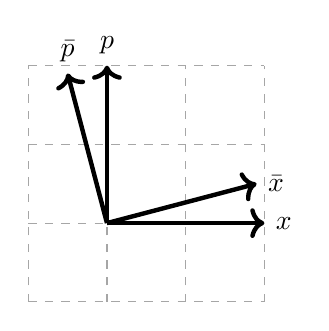
\begin{tikzpicture}
			\draw[help lines, color=gray!70, dashed] (-1,-1) grid (2,2);
			\draw[->,ultra thick] (0,0)--(2,0) node[right]{$x$};
			\draw[->,ultra thick] (0,0)--(0,2) node[above]{$p$};
			\draw[->,ultra thick] (0,0)--(1.9,0.5) node[right]{$\bar x$};
			\draw[->,ultra thick] (0,0)--(-0.5,1.9) node[above]{$\bar p$};
		\end{tikzpicture}
		\end{center}
		The infinitesimal transformation is as follows:
		\begin{gather*}
			\bar x = x\cos\epsilon - p\sin\epsilon \approx x - \epsilon p \\
			\bar p = x\sin\epsilon + p\cos\epsilon \approx \epsilon x + p
		\end{gather*}
		We must verify if this transformation is canonical:
		\begin{gather*}
			\acomm{\bar x}{\bar p} = \sum_{k = x, p} \pqty{\pdv{\bar x}{q_k}\pdv{\bar p}{p_k} - \pdv{\bar x}{p_k}\pdv{\bar p}{q_k}} = 0
		\end{gather*}
		To find the generator, we must solve the following partial differential equations:
		\begin{gather*}
			\pdv{g}{p} = -p \longrightarrow g = -\frac{p^2}{2} + f(x) \\
			\pdv{g}{x} = -x \longrightarrow g = -\frac{x^2}{2} + h(p) \\
			\therefore g = -\pqty{\frac{p^2}{2} + \frac{x^2}{2}} = -\mathcal{H},\qq{so the generator is the negative of the Hamiltonian!}
		\end{gather*}
\end{chapter2}

\begin{chapter2}\label{prob: 11}
	
\end{chapter2}

\newtheorem{chapter4}{Exercise}
\newcounter{subpart4}[chapter4]

\chapter{The Postulates - A General Discussion}

\begin{chapter4}\label{prob: 1}
	\stepcounter{subpart4}
		(\arabic{subpart4})
		The possible values are the eigenvalues of $L_z$. Since $L_z$ is already diagonal, its eigenvalues are the diagonal elements 1, 0 and -1. \\\\
		\stepcounter{subpart4}
		(\arabic{subpart4})
		\begin{gather*}
			\ev{L_x} = \expval{L_x}{1} = 
			\begin{bmatrix}
				1 & 0 & 0
			\end{bmatrix}
			\frac{1}{\sqrt{2}}
			\begin{bmatrix}
				0 & 1 & 0 \\
				1 & 0 & 1 \\
				0 & 1 & 0
			\end{bmatrix}
			\begin{bmatrix}
				1 \\
				0 \\
				0 \\
			\end{bmatrix}
			= 0 \\
			\ev{L^2_x} = \ev{L^2_x}{1} = 
			\begin{bmatrix}
				1 & 0 & 0
			\end{bmatrix}
			\frac{1}{2}
			\begin{bmatrix}
				1 & 0 & 1 \\
				0 & 2 & 0 \\
				1 & 0 & 1
			\end{bmatrix}
			\begin{bmatrix}
				1 \\
				0 \\
				0 \\
			\end{bmatrix}
			= \frac{1}{2} \\
			\Delta L_x = \sqrt{\ev{L^2_x} - \ev{L_x}^2} = \frac{1}{\sqrt{2}}
		\end{gather*}
		\stepcounter{subpart4}
		(\arabic{subpart4})
		We must solve the eigenvalue problem for $L_x$:
		\begin{gather*}
			\frac{1}{\sqrt{2}}
			\begin{vmatrix}
				-\lambda & 1 & 0 \\
				1 & -\lambda & 1 \\
				0 & 1 & -\lambda
			\end{vmatrix}
			= \frac{1}{\sqrt{2}}[-\lambda(\lambda^2 -1) - (-\lambda)] = 0 \longrightarrow \lambda = 1, 0, -1
		\end{gather*}
		The eigenstates are found by substituting the eigenvalues and solving:
		\begin{gather*}
			\ket{L_x = 0} = \frac{1}{\sqrt{2}}
			\begin{bmatrix}
				1 \\
				0 \\
				-1
			\end{bmatrix}
			, \;\; \ket{L_x = 1} = \frac{1}{\sqrt{2}}
			\begin{bmatrix}
				1/\sqrt{2} \\
				1 \\
				1/\sqrt{2}
			\end{bmatrix}
			, \;\; \ket{L_x = -1} = \frac{1}{\sqrt{2}}
			\begin{bmatrix}
				1/\sqrt{2} \\
				-1 \\
				1/\sqrt{2}
			\end{bmatrix}
		\end{gather*}
		\stepcounter{subpart4}
		(\arabic{subpart4})
		The eigenstate $\ket{\psi}$ for the eigenvalue $L_z = -1$ is:
		\begin{gather*}
			\ket{\psi} = 
			\begin{bmatrix}
				0 \\
				0 \\
				1
			\end{bmatrix}
		\end{gather*}
		The probabilities are found by dotting the ket with the eigenbras corresponding to the eigenstates of $L_z$:
		\begin{gather*}
		 	P(L_x = 0) = |\braket{L_x = 0}{\psi}|^2 = \left|\frac{1}{\sqrt{2}}
		 	\begin{bmatrix}
		 		1 & 0 & -1
		 	\end{bmatrix}
		 	\begin{bmatrix}
		 		0 \\
		 		0 \\
		 		1
		 	\end{bmatrix}\right|^2
		 	= \frac{1}{2} \\
		 	P(L_x = 1) = |\braket{L_x = 1}{\psi}|^2 = \left|\frac{1}{\sqrt{2}}
		 	\begin{bmatrix}
		 		\frac{1}{\sqrt{2}} & 1 & \frac{1}{\sqrt{2}}
		 	\end{bmatrix}
		 	\begin{bmatrix}
		 		0 \\
		 		0 \\
		 		1
		 	\end{bmatrix}\right|^2
		 	= \frac{1}{4} \\
		 	P(L_x = -1) = |\braket{L_x = -1}{\psi}|^2 = \left|\frac{1}{\sqrt{2}}
		 	\begin{bmatrix}
		 		\frac{1}{\sqrt{2}} & -1 & \frac{1}{\sqrt{2}}
		 	\end{bmatrix}
		 	\begin{bmatrix}
		 		0 \\
		 		0 \\
		 		1
		 	\end{bmatrix}\right|^2
		 	= \frac{1}{4}
		\end{gather*}
		\stepcounter{subpart4}
		(\arabic{subpart4})
		$L^2_z$ is a degenerate matrix with eigenvalues $0, 1, 1$, so when the state is measured to be $L^2_z = 1$, the state after the measurement is an eigenspace in $\mathcal{V}^2$. The linearly independent eigenkets describing this eigenspace corresponding to the eigenvalue $L^2_z = 1$ are:
		\begin{gather*}
			\ket{\omega,1} =
			\begin{bmatrix}
				1 \\
				0 \\
				0
			\end{bmatrix}, \;\;
			\ket{\omega,2} =
			\begin{bmatrix}
				0 \\
				0 \\
				1 	
			\end{bmatrix} 
		\end{gather*}
		Constructing the projection operator for these eigenkets to find the normalised state and its probability after measurement:
		\begin{gather*}
			\mathbb{P}_{\omega} = \sum_i \op{\omega,i}{\omega,i} \\
			\ket{\psi '} = \frac{\mathbb{P}_{\omega}\ket{\psi}}{\abs{\braket{\mathbb{P}_{\omega}{\psi}}}} = \frac{2}{\sqrt 3}
			\begin{bmatrix}
				1/2 \\
				0 \\
				1/\sqrt{2} 	
			\end{bmatrix} \\
			P\pqty{L^2_z = 1 } = \expval{\mathbb{P}_{\omega}}{\psi} =
			\mel**{\begin{bmatrix}
				\frac{1}{2} & \frac{1}{2} & \frac{1}{\sqrt{2}}  	
			\end{bmatrix}}
			{\begin{bmatrix}
				1 \\
				0 \\
				0 \\
			\end{bmatrix}
			\begin{bmatrix}
				1 & 0 & 0  	
			\end{bmatrix}
			+
			\begin{bmatrix}
				0 \\
				0 \\
				1  	
			\end{bmatrix}
			\begin{bmatrix}
				0 & 0 & 1  	
			\end{bmatrix}}
			{\begin{bmatrix}
				1/2 \\
				1/2 \\
				1/\sqrt{2}  	
			\end{bmatrix}} \\
			= \begin{bmatrix}
				\frac{1}{2} & \frac{1}{2} & \frac{1}{\sqrt{2}}  	
			\end{bmatrix}
			\begin{bmatrix}
				1 & 0 & 0\\
				0 & 0 & 0\\
				0 & 0 & 1
			\end{bmatrix}
			\begin{bmatrix}
				1/2 \\
				1/2 \\
				1/\sqrt{2}  	
			\end{bmatrix}
			= \frac{3}{4}
		\end{gather*}
		The outcomes of measuring $L_z$ are its eigenvalues, which are $\omega_1 = 0, \omega_2 = 1, \omega_3 = -1$. Their respective probabilities are found by dotting the current state with their eigenvectors:
		\begin{gather*}
			P(L_z = 0) = \abs{\braket{\omega_1}{\psi '}}^2 =
			\pqty{\begin{bmatrix}
				 0 & 1 & 0
			\end{bmatrix}
			\frac{2}{\sqrt 3}
			\begin{bmatrix}
				1/2 \\
				0 \\
				1/\sqrt{2}
			\end{bmatrix}}^2 = 0 \\
			P(L_z = 1) = \abs{\braket{\omega_2}{\psi '}}^2 =
			\pqty{\begin{bmatrix}
				 1 & 0 & 0
			\end{bmatrix}
			\frac{2}{\sqrt 3}
			\begin{bmatrix}
				1/2 \\
				0 \\
				1/\sqrt{2}
			\end{bmatrix}}^2 = \frac{1}{3} \\
			P(L_z = -1) = \abs{\braket{\omega_3}{\psi '}}^2 =
			\pqty{\begin{bmatrix}
				 0 & 0 & 1
			\end{bmatrix}
			\frac{2}{\sqrt 3}
			\begin{bmatrix}
				1/2 \\
				0 \\
				1/\sqrt{2}
			\end{bmatrix}}^2 = \frac{2}{3}
		\end{gather*}
		\stepcounter{subpart4}
		(\arabic{subpart4})
		The probabilities for each of the eigenvalues of $L_z$ is:
		\begin{gather*}
			P(L_z = 0) = \abs{\braket{\omega_1}{\psi}}^2 = \frac{1}{2} = \abs{\alpha}^2 \\
			P(L_z = 1) = \abs{\braket{\omega_2}{\psi}}^2 = \frac{1}{4} = \abs{\beta}^2 \\
			P(L_z = 1) = \abs{\braket{\omega_3}{\psi}}^2 = \frac{1}{4} = \abs{\gamma}^2
		\end{gather*}
		The normalised state is thus:
		\begin{gather*}
			\ket{\psi} =  \frac{\alpha\ket{L_z = 0} + \beta\ket{L_z = 1} + \gamma\ket{L_z = -1}}{\sqrt{\abs{\alpha}^2 + \abs{\beta}^2 + \abs{\gamma}^2}} = \alpha\ket{L_z = 0} + \beta\ket{L_z = 1} + \gamma\ket{L_z = -1}
		\end{gather*}
		However, the most general state is:
		\begin{gather*}
			\ket{\psi} =  \frac{e^{i\delta_1}}{\sqrt{2}}\ket{L_z = 0} +\frac{e^{i\delta_2}}{2}\ket{L_z = 1} + \frac{e^{i\delta_3}}{2}\ket{L_z = -1}
		\end{gather*}
		This is because when performing measurements of other variables, interference terms come into play. For example, if we measure $L_x = 0$ in the given state:
		\begin{gather*}
			P(L_x = 0) = \abs{\braket{L_x = 0}{\psi}}^2 =
			\abs{\frac{1}{\sqrt{2}}
			\begin{bmatrix}
				1 & 0 & -1
			\end{bmatrix}
			\frac{1}{2}
			\begin{bmatrix}
				e^{i\delta_1} \\
				\sqrt{2}e^{i\delta_2} \\
				e^{i\delta_3}
			\end{bmatrix}}^2
			= \frac{1}{2}\sin^2\pqty{\frac{\delta_3 - \delta_1}{2}}
		\end{gather*}
		Evidently the state will depend on the phase difference $(\delta_3 - \delta_1)$. Clearly the exponential phase factors are relevant in measuring probabilities.
\end{chapter4}

\begin{chapter4}\label{prob: 2}
	The expectation value is given by:
		\begin{gather*}
			\ev{P} = \ev{P}{\psi} = \int_{-\infty}^{\infty} \braket{\psi}{k}\mel*{k}{P}{\psi}\dd{k} =  \int_{-\infty}^{\infty}p\psi^*(k)\psi(k)\dd{k} \\
			\psi(k) = \braket{k}{\psi} = \int_{-\infty}^{\infty} \braket{k}{x}\braket{x}{\psi}\dd{x} = \frac{1}{\sqrt{2\pi}}\int_{-\infty}^{\infty} e^{-ikx}\psi(x)\dd{x} \\
			\psi^*(k) = \frac{1}{\sqrt{2\pi}} \int_{-\infty}^{\infty} e^{ikx}\psi^*(x) \dd{x} = \psi(-k), \;\; \because \psi^*(x) = \psi(x) \\
			\ev{P} = \int_{-\infty}^{\infty} \hbar k \;\psi(-k)\psi(k) \dd{k} = 0, \;\;\because\qq*{the integral is odd}
		\end{gather*}
\end{chapter4}

\begin{chapter4}\label{prob: 3}
	
\end{chapter4}

\begin{chapter4}\label{prob: 4}
	
\end{chapter4}

\newtheorem{chapter5}{Exercise}
\newcounter{subpart5}[chapter5]

\chapter{Simple Problems in One Dimension}

\begin{chapter5}\label{prob: 1}
	This can be solved by substitution:
		\begin{gather*}
			p = \pm\sqrt{2mE} \longrightarrow \dd{p} = \pm\frac{m}{\sqrt{2mE}}\dd{E}
		\end{gather*}
		Since there are two values that $p$ can take, we must expand the integral to include the values with respect to $E$:
		\begin{gather*}
			U(t) = \int_{-\infty}^0 -\frac{m}{\sqrt{2mE}} \op{E,-} e^{-iEt/\hbar} \dd{E} + \int_{0}^{\infty} \frac{m}{\sqrt{2mE}} \op{E,+} e^{-iEt/\hbar} \dd{E} \\
			U(t) = \sum_{\alpha = \pm} \int_{0}^{\infty} \frac{m}{\sqrt{2mE}} \op{E,\alpha} e^{-iEt/\hbar} \dd{E}
		\end{gather*}
\end{chapter5}

\begin{chapter5}\label{prob: 2}
	Using $\ket x$ as a trial solution:
		\begin{gather*}
			\frac{P^2}{2m}\ket{x} = E\ket{x} \\
			-\frac{\hbar^2}{2m}\pdv[2]{x}\ket{x} = E\ket{x} \\
			\pqty{\frac{\hbar^2}{2m}\dv[2]{x} + E}\ket{x} = 0
		\end{gather*}
		The solution to this differential equation is readily found by substituting $D = \dv{x}$ and solving the algebraic equation, giving:
		\begin{gather*}
			D = \pm \frac{ip}{\hbar} \longrightarrow \psi_E(x) = \frac{\beta}{\sqrt{2\pi\hbar}}\exp(\frac{ip}{\hbar}x) + \frac{\gamma}{\sqrt{2\pi\hbar}}\exp(-\frac{ip}{\hbar}x), \;\; p = \sqrt{2mE}
		\end{gather*}
		If $E \leq 0$, then the function consists of real exponentials that blow up at large values of $x$, and are thus not in the Hilbert space.
\end{chapter5}

\begin{chapter5}\label{prob: 3}
	We have the propagator and initial state:
		\begin{gather*}
			U(t) = \exp[\frac{i}{\hbar}\pqty{\frac{\hbar^2 t}{2m}\dv[2]{x}}] = \sum_{n=0}^{\infty} \frac{1}{n!}\pqty{\frac{i\hbar t}{2m}}^n \dv[2n]{x}, \;\;\; \psi(x,0) = \frac{e^{-x^2/2}}{\sqrt[4]\pi} \\
			\qq*{Expanding the initial state as a power series:}\psi(x,0) = \frac{1}{\sqrt[4]\pi} \sum_{n=0}^{\infty} \frac{(-1)^n x^{2n}}{n!(2)^n} \\
			\psi(x,t) = \pqty{\sum_{k=0}^{\infty} \frac{1}{k!}\pqty{\frac{i\hbar t}{2m}}^k \dv[2k]{x}}\pqty{\sum_{n=0}^{\infty}\frac{1}{\sqrt[4]\pi}\frac{(-1)^n x^{2n}}{n!(2)^n}} \\
			\psi(x,t) = \frac{1}{\sqrt[4]\pi}\bqty{\sum_{n=0}^{\infty}\sum_{k=0}^{n}\pqty{\frac{i\hbar t}{m}}^k\frac{\pqty{-1}^n}{n!k! (2)^{n+k}}\frac{\pqty{2n}!}{\pqty{2n-2k}!}x^{2(n-k)}}
		\end{gather*}
		The coefficients of the $x^{2n}$ terms are:
		\begin{gather*}
			x^0\colon \frac{(-1)^0}{0!}\bqty{1 - \frac{1}{2}\frac{i\hbar t}{m} + \frac{3}{8}\pqty{\frac{i \hbar t}{m}}^2 - \frac{5}{16}\pqty{\frac{i \hbar t}{m}}^3 + \frac{35}{128}\pqty{\frac{i \hbar t}{m}}^4 - ...}\frac{x^{2\times 0}}{2^0} \\
			x^2\colon \frac{(-1)^1}{1!}\bqty{1 - \frac{3}{2}\pqty{\frac{i \hbar t}{m}} + \frac{15}{8}\pqty{\frac{i \hbar t}{m}}^2 - \frac{35}{16}\pqty{\frac{i \hbar t}{m}}^3 + ...}\frac{x^{2 \times 1}}{2^1} \\
			x^4\colon \frac{(-1)^2}{2!}\bqty{1-\frac{5}{2}\pqty{\frac{i \hbar t}{m}} + \frac{35}{8}\pqty{\frac{i \hbar t}{m}}^2 - ...}\frac{x^{2 \times 2}}{2^2} \\
			\psi(x,t) = \frac{1}{\sqrt[4]{\pi}} \bqty{\sum_{n = 0}^{\infty} \frac{(-1)^n}{n!}\Bqty{1 - \pqty{n + \frac{1}{2}}\pqty{\frac{i \hbar t}{m}} + \frac{1}{2!}\pqty{n + \frac{1}{2}}\pqty{n + \frac{3}{2}}\pqty{\frac{i \hbar t}{m}}^2 - ...}\frac{x^{2n}}{2^n}} \\
			\psi(x,t) = \frac{1}{\sqrt[4]\pi} \bqty{\sum_{n = 0}^{\infty} \frac{(-1)^n}{n!}\pqty{1 + \frac{i \hbar t}{m}}^{-n-\frac{1}{2}} \frac{x^{2n}}{2^n}} \\ = \frac{1}{\sqrt{\sqrt{\pi}\pqty{1 + \frac{i \hbar t}{m}}}} \exp\bqty{-\frac{x^2}{2\pqty{1 + \frac{i \hbar t}{m}}}}
		\end{gather*}
\end{chapter5}

\begin{chapter5}\label{prob: 4}
	
\end{chapter5}

\end{document}